% !TeX spellcheck = nl_NL

\documentclass[11pt]{report}
\usepackage{./../hva}
\usepackage{./portfolio}

\titleMain{Portfolio}
\titleSub{\textit{Mistakes are made. Lessons are learned.}}

\begin{document}
	\maketitle
	\tableofcontents
	
	\chapter{Professioneel vakmanschap}
	\newpage
	% !TeX spellcheck = nl_NL

\competentie
{% competentieformulier
	\competentieformulier
	{% toelichting
		Je hebt kennis en vaardigheden die belangrijk zijn voor jouw rol als professional in het ICT-werkveld. Je kunt de kennis die je hebt opgedaan beoordelen op relevantie. Op basis daarvan maak je keuzes voor het toepassen ervan bij het uitvoeren en oplossen van praktijkvraagstukken. Je hanteert daarbij een methodische werkwijze, stelt criteria op waaraan het resultaat moet voldoen en werkt volgens professionele (internationale) ICT-standaarden. Je hebt een ondernemende houding.
	}
	{% deelcompetenties
		planmatig werken,%
		toepassing van (wetenschappelijke) kennis en inzichten,%
		kwaliteit leveren,%
		ondernemen%
	}
	{% beroepstaken
		1...,%
		2...,%
		Etc.%
	}
	{%
		Bewijs uit stage
	}
	{%
		Voor deze competentie mag je maximaal drie beroepsproducten opnemen als bewijs. Je mag één beroepsproduct vervangen door een ervaringsverslag. De beroepsproducten worden voorafgegaan door een toelichting in de vorm van een STARR-formulier. Een eventueel ervaringsverslag maak je ook door het STARR-formulier in te vullen.
	}
	{% verwijzing naar bewijs
		Bewijs 1,%
		Bewijs 2,%
		Bewijs 3%
	}
}
{% bewijzen
	\bewijs
	{% naam
		a
	}
	{% starr
		\starr
		{% betreft
			b
		}
		{% datum
			c
		}
		{% situatie
			d
		}
		{% taak
			e
		}
		{% activiteiten
			f
		}
		{% resultaat
			g
		}
		{% reflectie
			h
		}
	}
	{% bewijs
		
	},
	\bewijs
	{% naam
		a
	}
	{% starr
		\starr
		{% betreft
			b
		}
		{% datum
			c
		}
		{% situatie
			d
		}
		{% taak
			e
		}
		{% activiteiten
			f
		}
		{% resultaat
			g
		}
		{% reflectie
			h
		}
	}
	{% bewijs
		
	},
	\bewijs
	{% naam
		a
	}
	{% starr
		\starr
		{% betreft
			b
		}
		{% datum
			c
		}
		{% situatie
			d
		}
		{% taak
			e
		}
		{% activiteiten
			f
		}
		{% resultaat
			g
		}
		{% reflectie
			h
		}
	}
	{% bewijs
		
	}
}

	\newpage
	
	\chapter{Onderzoekend vermogen}
	\newpage
	% !TeX spellcheck = nl_NL

\competentie
{% competentieformulier
	\competentieformulier
	{% toelichting
		Je bent onderzoekend en brengt verschillende aspecten van een vraagstuk of probleem vanuit verschillende perspectieven in kaart. Je verzamelt relevante informatie uit erkende bronnen. Je analyseert deze informatie en brengt deze op systematische wijze met elkaar in verband. Op basis hiervan vorm je een oordeel en kom je tot een oplossing. Je kunt verschillende invalshoeken gebruiken om tot nieuwe ideeën en oplossingen te komen.
	}
	{% deelcompetenties
		analyse en oordeelsvorming,%
		onderzoeken,%
		creativiteit%
	}
	{% beroepstaken
		1...,%
		2...,%
		Etc.%
	}
	{%
		Bewijs uit stage
	}
	{%
		Deze competentie moet je verplicht aantonen tijdens het assessment. Voor onderzoekend vermogen is het met een voldoende beoordeelde onderzoeksrapport een verplicht bewijs. Naast het onderzoeksrapport mag je nog een ander bewijs selecteren: een beroepsproduct of een ervaringsverslag in de vorm van een ingevuld STARR-formulier. Het onderzoeksverslag wordt voorafgegaan door een toelichting in de vorm van een STARR-formulier. Als je nog een beroepsproduct toe voegt, wordt dit ook voorafgegaan door een toelichting in de vorm van een STARR-formulier.
	}
	{% verwijzing naar bewijs
		Onderzoeksrapport,%
		Bewijs 2%
	}
}
{% bewijzen
	\bewijs
	{% naam
		Onderzoeksrapport
	}
	{% starr
		\starr
		{% betreft
			b
		}
		{% datum
			c
		}
		{% situatie
			d
		}
		{% taak
			e
		}
		{% activiteiten
			f
		}
		{% resultaat
			g
		}
		{% reflectie
			h
		}
	}
	{% bewijs
		{%
			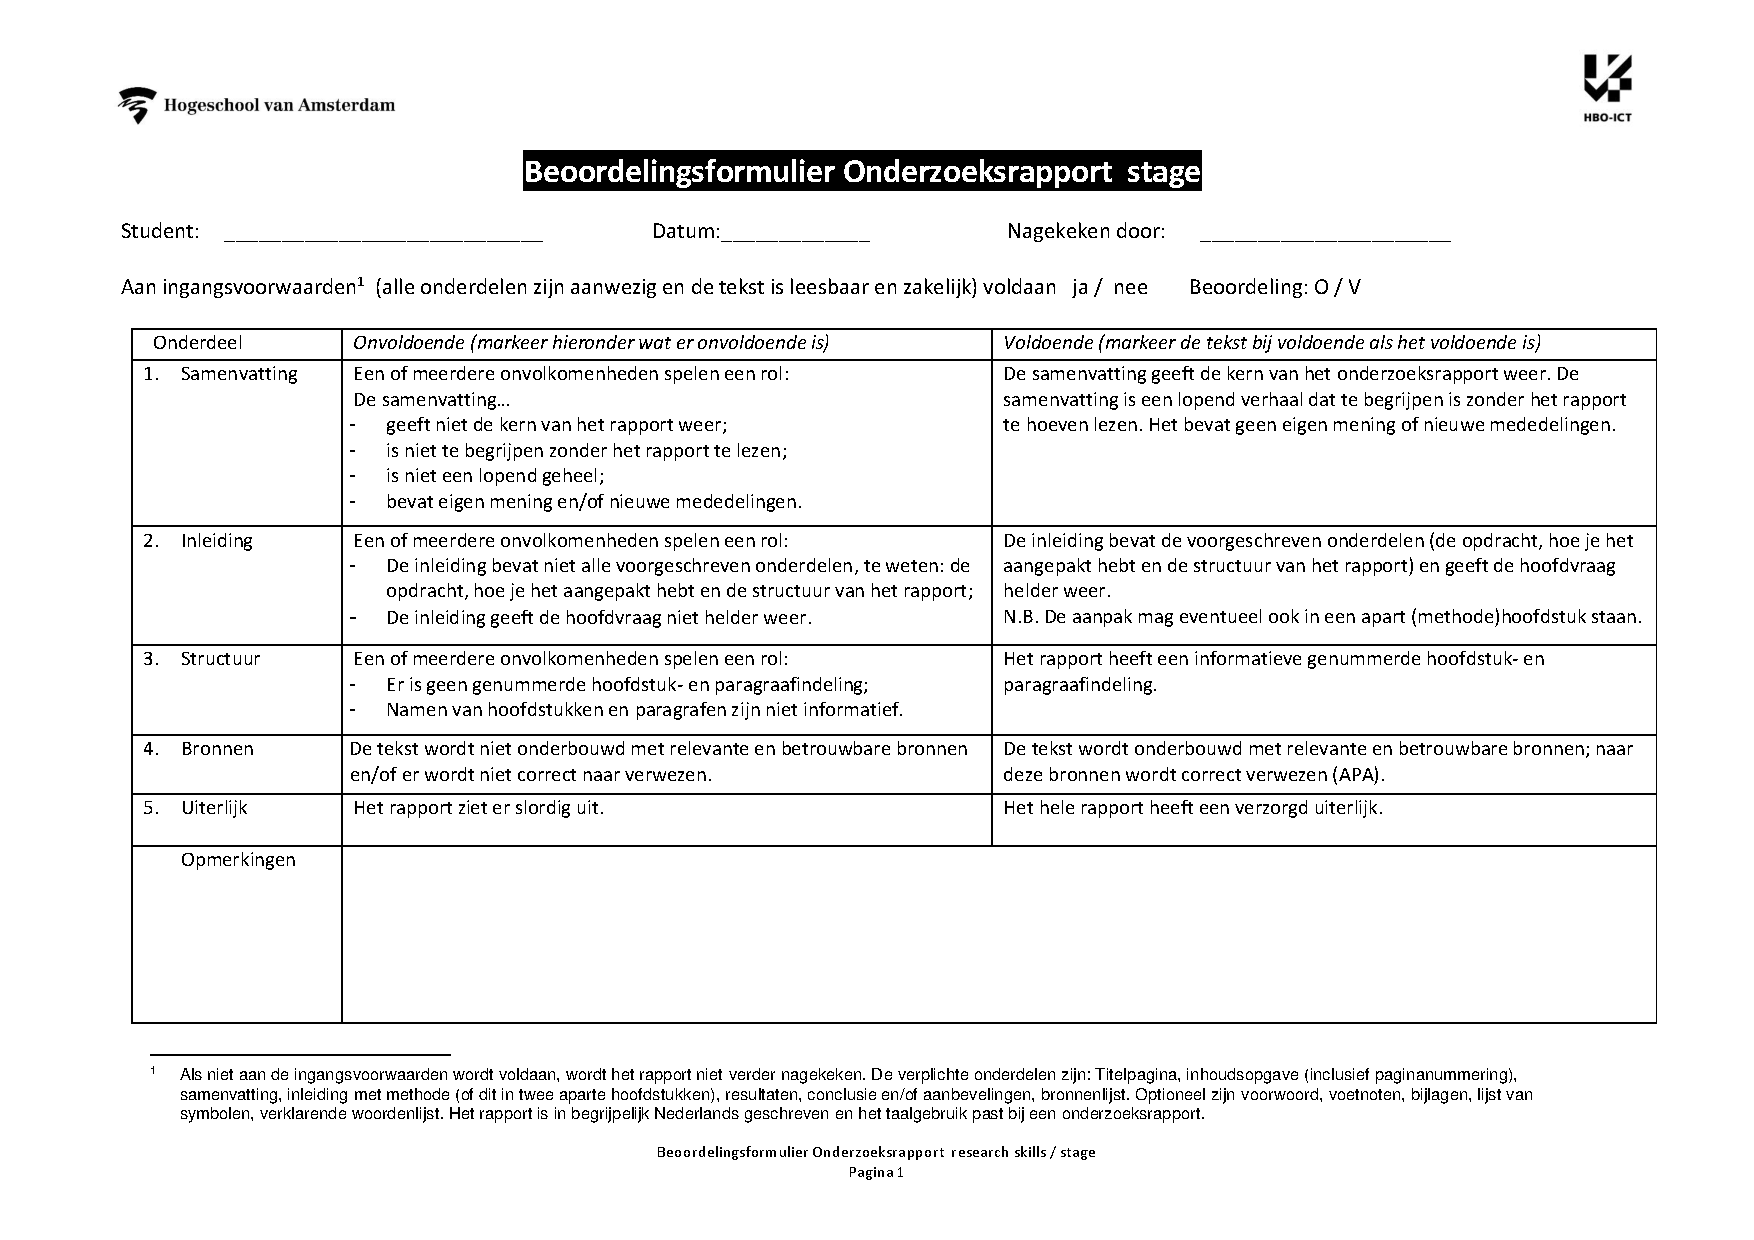
\includepdf[
				pages=1,
				frame,
				scale=0.90,
				pagecommand={
					\section*{Bewijs}
					Zie \autoref{appendix:Onderzoeksrapport} voor het onderzoeksrapport.
				}
			]{./appendices/beoordelingsformulier-onderzoeksrapport}
			
			\includepdf[
				pages=2-,
				frame,
				scale=0.90,
				pagecommand={}
			]{./appendices/beoordelingsformulier-onderzoeksrapport}
		}
	},
	\bewijs
	{% naam
		a
	}
	{% starr
		\starr
		{% betreft
			b
		}
		{% datum
			c
		}
		{% situatie
			d
		}
		{% taak
			e
		}
		{% activiteiten
			f
		}
		{% resultaat
			g
		}
		{% reflectie
			h
		}
	}
	{% bewijs
		
	}
}

	\newpage
	
	\chapter{Leervermogen}
	\newpage
	% !TeX spellcheck = nl_NL

\competentie
{% competentieformulier
	\competentieformulier
	{% toelichting
		Je bent in staat om op je eigen handelen te reflecteren en daarin sterke en minder sterke kanten te benoemen. Je staat open voor de visie en feedback van anderen en geeft sturing aan je eigen ontwikkeling als ICT-professional.
	}
	{% deelcompetenties
		reflecteren,%
		zelfsturing%
	}
	{% beroepstaken
		1...,%
		2...,%
		Etc.%
	}
	{%
		Bewijs uit stage
	}
	{%
		Deze competentie moet je verplicht aantonen tijdens het assessment. Voor leervermogen zijn  je COP (competentie-ontwikkelplan) en je tussentijdse en eindevaluatie verplicht bewijs. Dit zijn geen beroepsproducten en daarom hoef je bij dit bewijs geen STARR toe te voegen, dat geldt ook voor als je feedbackformulieren ingevuld door collega’s en een analyse daarvan als bewijs wilt gebruiken. Je zou ook een ervaringsverslag in de vorm van een STARR-formulier kunnen schrijven.
	}
	{% verwijzing naar bewijs
		COP,%
		Tussentijdse evaluatie door bedrijfsbegeleider,%
		Eindevaluatie door bedrijfsbegeleider%
	}
}
{% bewijzen
	\bewijs
	{% naam
		COP
	}
	{}
	{% bewijs
		
	},
	\bewijs
	{% naam
		Tussentijdse evaluatie door bedrijfsbegeleider
	}
	{}
	{% bewijs
		
	},
	\bewijs
	{% naam
		Eindevaluatie door bedrijfsbegeleider
	}
	{}
	{% bewijs
		
	}
}

	\newpage
	
	\chapter{Communicatief vermogen}
	\newpage
	% !TeX spellcheck = nl_NL

\competentie
{% competentieformulier
	\competentieformulier
	{% toelichting
		Je bent sensitief, toegankelijk en overtuigend in je communicatie met uiteenlopende doelgroepen, waaronder klanten. Je neemt de vraag van de klant als uitgangspunt, maakt duidelijke afspraken en checkt of steeds aan de verwachtingen is voldaan.
	}
	{% deelcompetenties
		communiceren,%
		rapporteren,%
		klantgerichtheid%
	}
	{% beroepstaken
		1...,%
		2...,%
		Etc.%
	}
	{%
		Bewijs
	}
	{%
		Voor communicatief vermogen is je beoordelingsformulier van de stagepresentatie een verplicht bewijs. Naast het beoordelingsformulier mag je nog een ander bewijs selecteren (beroepsproduct of ervaringsverslag in de vorm van een ingevuld STARR-formulier). Elk beroepsproduct wordt voorafgegaan door een toelichting in de vorm van een STARR-formulier.
	}
	{% verwijzing naar bewijs
		Beoordelingsformulier van de stagepresentatie,%
		Bewijs 2%
	}
}
{% bewijzen
	\bewijs
	{% naam
		Beoordelingsformulier van de stagepresentatie
	}
	{}
	{% bewijs
		
	},
	\bewijs
	{% naam
		a
	}
	{% starr
		\starr
		{% betreft
			b
		}
		{% datum
			c
		}
		{% situatie
			d
		}
		{% taak
			e
		}
		{% activiteiten
			f
		}
		{% resultaat
			g
		}
		{% reflectie
			h
		}
	}
	{% bewijs
		
	}
}

	\newpage
	
	\chapter{Beroepsethiek en maatschappelijke oriëntatie}
	\newpage
	% !TeX spellcheck = nl_NL

\competentie
{% competentieformulier
	\competentieformulier
	{% toelichting
		Je weet wat er in de samenleving speelt en houdt daar rekening bij het uitvoeren van het werk. Je bent je bewust van de betekenis van aangeleerde kennis en vaardigheden in de maatschappelijke context. Je beschikt over het vermogen om kennis kritisch te toetsen en te handelen volgens de geldende (beroeps)normen. 
	}
	{% deelcompetenties
		maatschappelijke verantwoordelijkheid,%
		beroepsethiek (bijvoorbeeld privacy en security aspecten)%
	}
	{% beroepstaken
		1...,%
		2...,%
		Etc.%
	}
	{%
		Bewijs
	}
	{%
		Kies één of twee bewijzen bij beroepsethiek en maatschappelijke oriëntatie. Bij deze competentie mogen beide bewijzen ervaringsverslagen zijn in de vorm van een ingevuld STARRR-formulier. Als je toch een beroepsproduct  hebt, wordt dat voorafgegaan door een toelichting in de vorm van een STARR-formulier.
	}
	{% verwijzing naar bewijs
		Bewijs 1,%
		Bewijs 2%
	}
}
{% bewijzen
	\bewijs
	{% naam
		a
	}
	{% starr
		\starr
		{% betreft
			b
		}
		{% datum
			c
		}
		{% situatie
			d
		}
		{% taak
			e
		}
		{% activiteiten
			f
		}
		{% resultaat
			g
		}
		{% reflectie
			h
		}
	}
	{% bewijs
		
	},
	\bewijs
	{% naam
		a
	}
	{% starr
		\starr
		{% betreft
			b
		}
		{% datum
			c
		}
		{% situatie
			d
		}
		{% taak
			e
		}
		{% activiteiten
			f
		}
		{% resultaat
			g
		}
		{% reflectie
			h
		}
	}
	{% bewijs
		
	}
}

	\newpage
		
	\chapter{Samenwerken}
	\newpage
	% !TeX spellcheck = nl_NL

\competentie
{% competentieformulier
	\competentieformulier
	{% toelichting
		Je bent in je samenwerking met collega’s zowel taak- als teamgericht om resultaten zo efficiënt en effectief mogelijk te realiseren. Je kunt functioneel leiding geven aan een (project)team en teamleden stimuleren en motiveren. Je werkt goed samen met de klant. 
	}
	{% deelcompetenties
		samenwerken,%
		leidinggeven%
	}
	{% beroepstaken
		1...,%
		2...,%
		Etc.%
	}
	{%
		Bewijs
	}
	{%
		Kies één of twee bewijzen bij samenwerken. Bij samenwerken gaat het om ervaringsverslagen in de vorm van een ingevuld STARR-formulier.
	}
	{% verwijzing naar bewijs
		Bewijs 1,%
		Bewijs 2%
	}
}
{% bewijzen
	\bewijs
	{% naam
		a
	}
	{% starr
		\starr
		{% betreft
			b
		}
		{% datum
			c
		}
		{% situatie
			d
		}
		{% taak
			e
		}
		{% activiteiten
			f
		}
		{% resultaat
			g
		}
		{% reflectie
			h
		}
	}
	{% bewijs
		
	},
	\bewijs
	{% naam
		a
	}
	{% starr
		\starr
		{% betreft
			b
		}
		{% datum
			c
		}
		{% situatie
			d
		}
		{% taak
			e
		}
		{% activiteiten
			f
		}
		{% resultaat
			g
		}
		{% reflectie
			h
		}
	}
	{% bewijs
		
	}
}

	\newpage
	
	% Seperate the appendix TOC from the main content TOC
	\addtocontents{toc}{\protect\newpage}
	\addtocontents{toc}{\protect\chapter*{Appendices}}
	
	\renewcommand\appendixname{Appendix}
	
	\appendix
	\chapter{Curriculum Vitae}
\label{appendix:CurriculumVitae}
\newpage
\pdfpa{cv}
\newpage

\chapter{Beroepstaken}
\label{appendix:Beroepstaken}
\newpage
\pdfpa{beroepstaken}
\newpage

\chapter{Onderzoeksrapport}
\label{appendix:Onderzoeksrapport}
\newpage
\pdfpa{onderzoeksrapport}
\newpage

\end{document}
